\chapter{Technical Evaluation}
\label{chap:technical-evaluation}
\centerline{\rule{149mm}{.02in}}
\vspace{2cm}

We have shown that the point $kd$-tree greatly outperforms the Pyramid tree for the two scientific datasets. For all synthetic data and the 3D point cloud dataset, the Pyramid tree is faster, especially with regard to point deletion.

This chapter will explore the reasons for this, determining what characteristics the astrophysics dataset cause the performance of the structures to degenerate. The chapter will conclude by discussing the types of data suitable for the Pyramid Tree and $kd$-tree, along with some further discussion on the implications of the results from this evaluation.

\section{Characteristics of Astrophysics Dataset}
\label{sec:data-characteristics}

A dataset is considered \textit{skewed} if a greater number of points are present in certain regions of the data space than other regions of the space. That is, the underlying frequency or probability distribution of point locations is non-uniform. Intuitively, the skewness of a dataset increases as the \textit{difference} between the frequency/probability of points in different spatial regions increases. That is, some regions of the data space are denser than others.

Histograms are used to visualise the frequency distributions of one-dimensional data. Since this project deals with multi-dimensional data, multiple histograms, one for each dimension, can be produced to gain insight into point distribution. The astrophysics dataset was computed using a 3D sampling lattice, computing ten fields at each point. The original simulation imposes uses interpolation between points in the sampling lattice \cite{astrophysics-dataset}. Carr et al. discusses how this interpolation ``implicitly applies the spatial relation between sample points" and shows that histograms are equivalent to nearest-neighbour interpolation \cite{histograms-and-isosurfaces}. This means histograms poorly represent datasets that use higher-order interpolants, such as the astrophysics dataset, because they ``over-emphasizes densely-sampled regions and under-emphasizes sparsely-sampled regions" \cite{histograms-and-isosurfaces}. 

Isosurface statistics have been proposed as a superior representation of datasets \cite{histograms-and-isosurfaces}. They are conceptually and computationally more complex to compute however. Due to project time constraints, isosurface statistics shall not be used. While histograms are poorer representation of the data, the aim of this evaluation is determine the magnitude of the skew present in the different dimensions of the dataset. Histograms still provide a visual representation of data distribution, even if it is not as accurate as desired. Therefore, histograms will be used to visualise the distribution of the astrophysics dataset.

\begin{figure}
	\begin{center}
		\begin{subfloat}[Dimension 1 (total particle density)]{%
			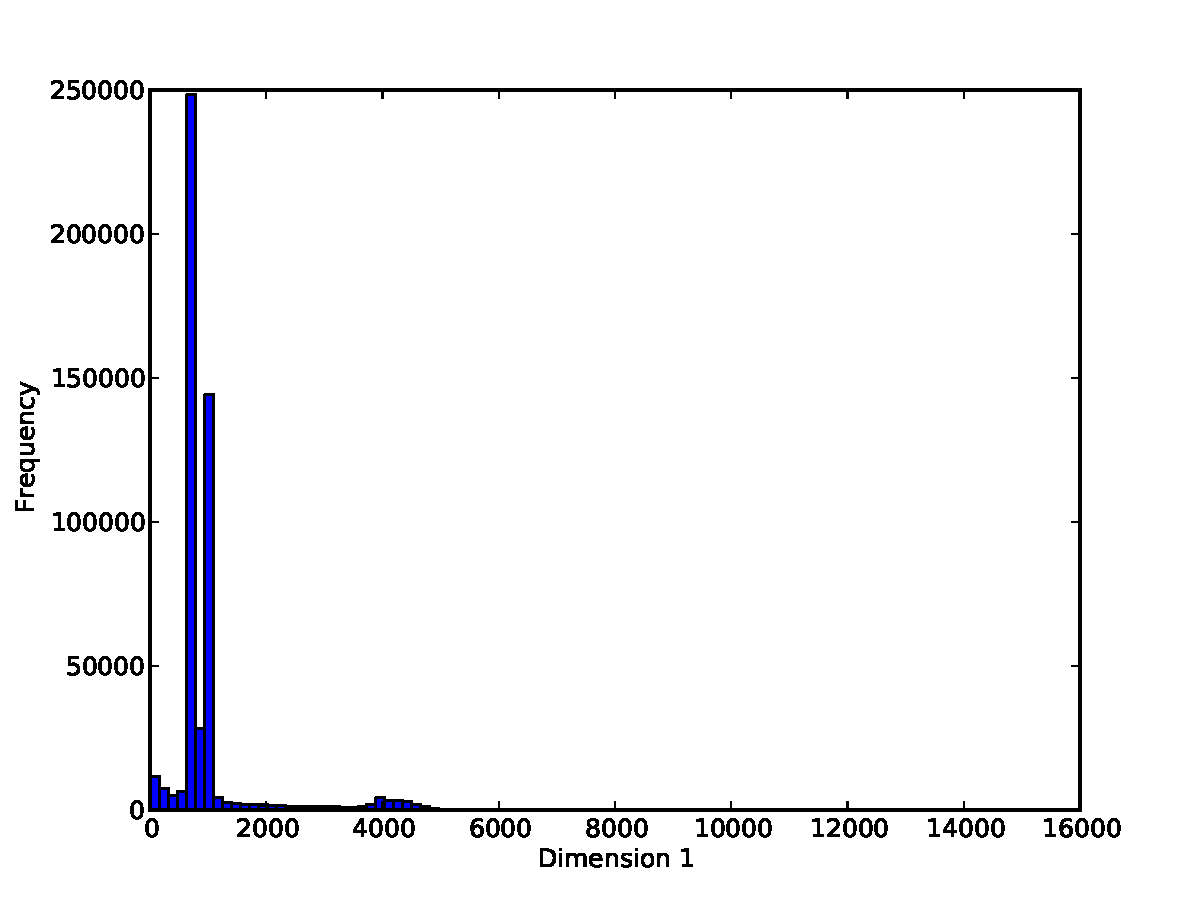
\includegraphics[scale=0.36]{figures/histograms/astrophysics_500000_0.pdf}
		}
		\end{subfloat}~
		\begin{subfloat}[Dimension 2 (gas temperature)]{%
			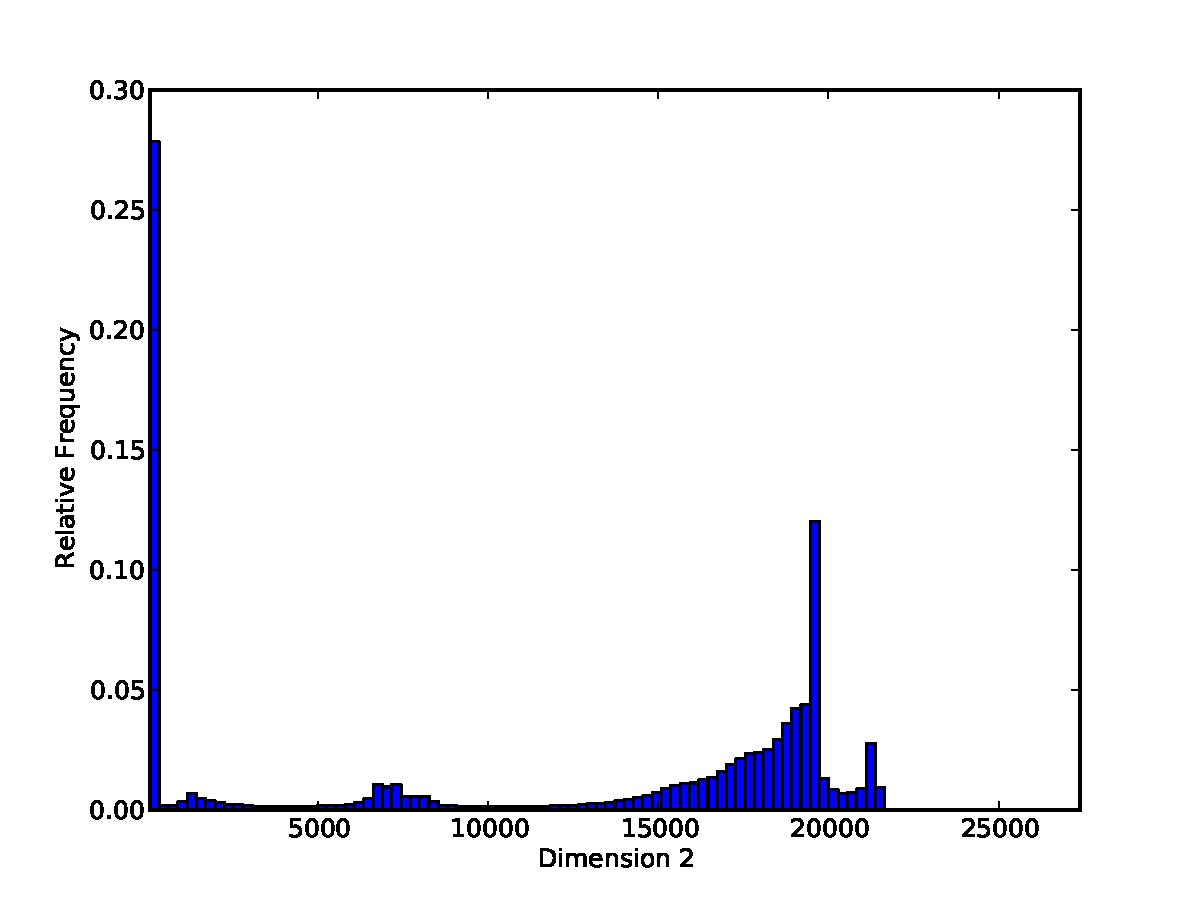
\includegraphics[scale=0.36]{figures/histograms/astrophysics_500000_1.pdf}
		}
		\end{subfloat}
	\end{center}

	\caption{Frequency Distributions of Dimensions 1 and 2 of Astrophysics Dataset}
	\label{fig:astrophysics-histograms1}
\end{figure}

\begin{figure}
	\begin{center}
		\begin{subfloat}[Dimension 3 (H mass abundance)]{%
			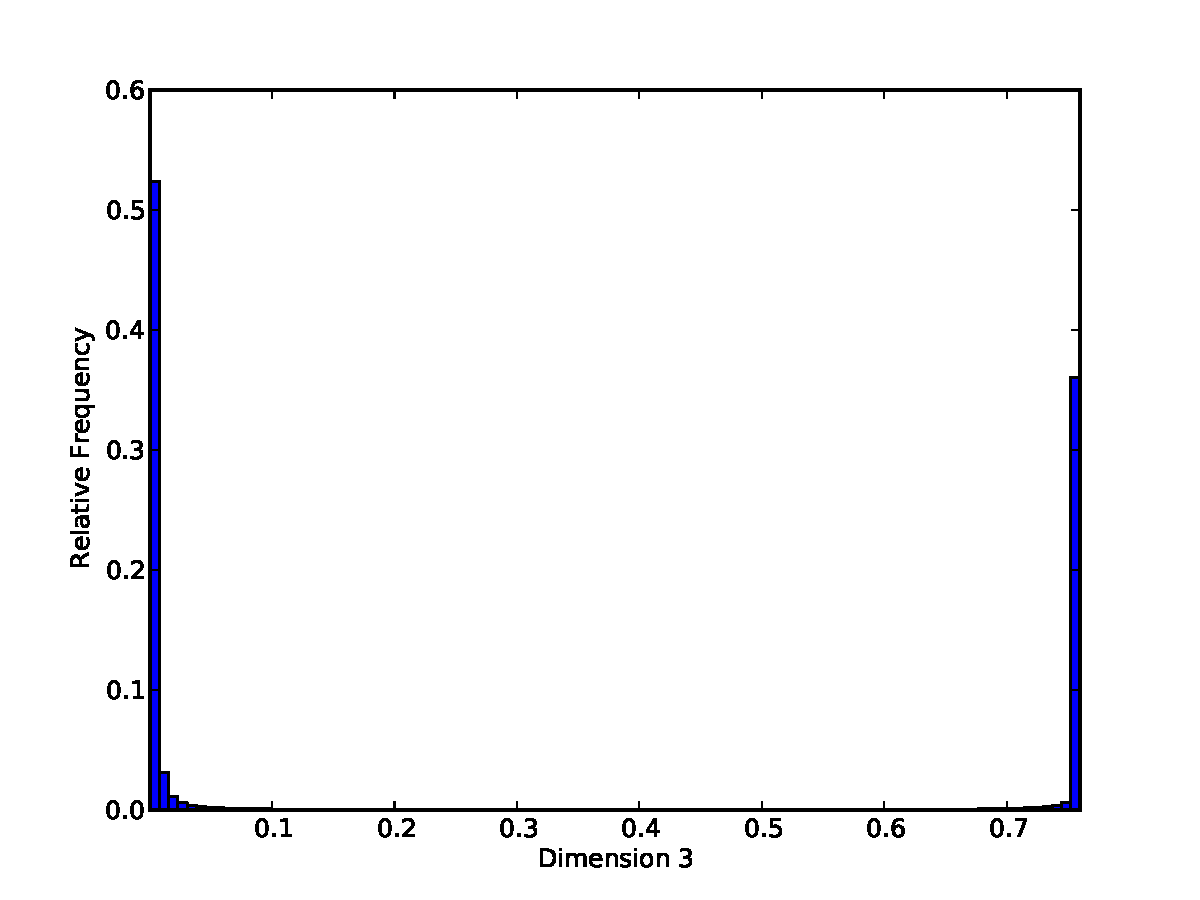
\includegraphics[scale=0.36]{figures/histograms/astrophysics_500000_2.pdf}
		}
		\end{subfloat}~
		\begin{subfloat}[Dimension 7 (He${}^{++}$ mass abundance)]{%
			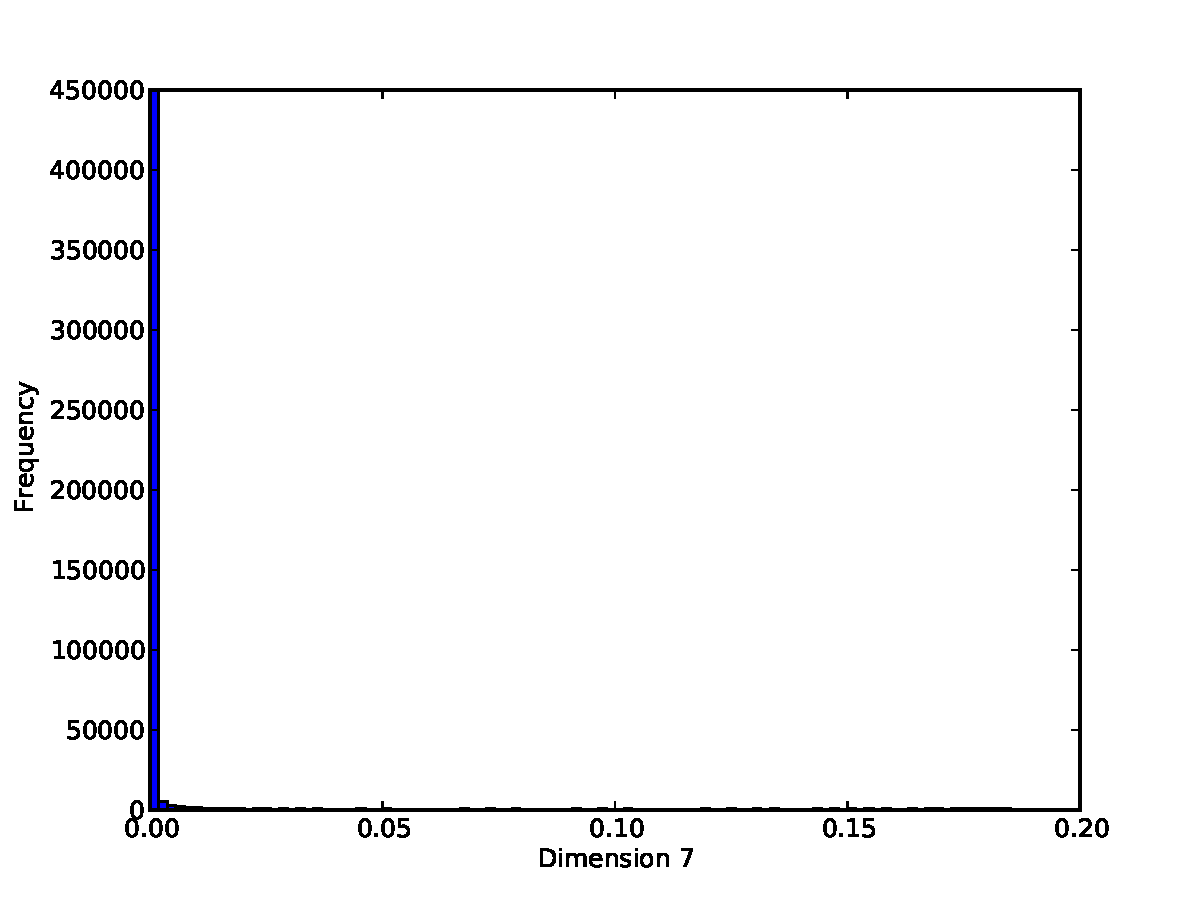
\includegraphics[scale=0.36]{figures/histograms/astrophysics_500000_6.pdf}
		}
		\end{subfloat}
	\end{center}

	\caption{Frequency Distributions of Dimensions 3 and 7 of Astrophysics Dataset}
	\label{fig:astrophysics-histograms2}
\end{figure}

Ten histograms have been generated using each dimension of the sampled astrophysics dataset used for performance analyses in Chapter \ref{chap:design-and-implementation}. Figures \ref{fig:astrophysics-histograms1} and \ref{fig:astrophysics-histograms2} show histograms of dimensions 1, 2, 3 and 7. The histograms for the remaining dimensions are provided in Appendix \ref{sec:app-histograms} since they have distributions similar to the dimensions shown here and thus, add little information. Using these histograms, the following observations can be made:
\begin{enumerate}
	\item the first two dimensions, total particle density and gas temperature, appear to have the greatest variance, although there are still very large peaks
	\item the majority of points are clustered on the lower or upper boundaries of dimensions 3, 4, 5 and 6. The respective histograms have massive peaks at either end of the distribution and much smaller peaks in-between
	\item the majority of the points are clustered on the lower boundary of dimensions 7, 8, 9 and 10 (single large peak at lower boundary)
\end{enumerate}
The astrophysics dataset is therefore highly skewed, since most points are clustered at the boundaries of the dimensions. It follows that the vast majority of the data space has little to no points, making the dataset \textit{sparse}.

\section{Effect of Distribution on Pyramid Tree}

We now explore the effect of the highly skewed distribution on the Pyramid Tree. Recall that the Pyramid Tree maps a point $v$ to a single scalar named the Pyramid value $pv_v$. Points with the same Pyramid value are stored in the same bucket. Table \ref{tab:final-bucket-size} shows bucket size statistics and how long it takes to query all the points for the sampled astrophysics dataset, when different dimensions are used. When only dimensions 1 and 2, the dimensions with the greatest variance, are used, average bucket size decreases substantially. Dimensions 3 and 7 have larger clusters of points close together, so they cause the average bucket size to increase.

The histograms from Section \ref{sec:data-characteristics} illustrate how most points lie on, or close to, the boundaries of the dataset. This is a significant problem for the Pyramid Tree because it always chooses the dimension whose distance from the centre point of the data is the highest. If a large number of points are on a dimensional boundary, then its likely the same dimension will be chosen. Since each point will the same coordinate value for the chosen dimension, because they are on the same boundary, they will have the same pyramid value.

\begin{table}
	\centering
	\makebox[\textwidth][c]{%
		\begin{tabular}{|l|l|l|l|l|}
			\hline
			\textbf{Dimensions} & \textbf{Time to Query (sec)} & \textbf{Average} & \textbf{Max} & \textbf{\#Buckets} \\
			\hline
			All & 60.0216 & 3586.57 & 235260 & 120 \\
			1 and 2 & 0.0713558 & 6.52433 & 102 & 25232 \\
			3 and 7 & 8.30587 & 89.2853 & 141235 & 3056 \\
			\hline
			No Boundary Coordinates & 27.6034 & 25.3722 & 45031 & 16963 \\
			\hline
		\end{tabular}
	}%
	\caption{Pyramid Tree Bucket Size Statistics with Different Dimensions of Astrophysics Dataset}
	\label{tab:final-bucket-size}
\end{table}

Histograms are equivalent to nearest-neighbour interpolation, so they do not show if the points inside the bins at the boundary of the graphs are \textit{actually} boundary values or just close to the boundary. To determine if clusters of points at boundaries is truly the main cause of large buckets, a heuristic called \textbf{No Boundary Coordinates} was developed. Let $v$ be a point and $min_i$ and $max_i$ be the minimum and maximum boundary values for dimension $i \in \lbrace 0, 1, ..., d - 1 \rbrace$. Let $j$ be the dimension $v$ is furthest from the centre point. If $v_j = min_j$ or $v_j = max_j$, then a new dimension $k$ is chosen, such that $v_k$ is the \textit{second} furthest coordinate from the centre point. If $v_k$ is at the boundary, then the next furthest is chosen again. This process is repeated until a coordinate which is not on a boundary is found. If all coordinates are on a boundary, then the first dimension is chosen.

Table \ref{tab:final-bucket-size} shows how this simple heuristic causes performance to increase by decreasing average bucket size. However, it is still significantly slower than the $kd$-tree, so other kinds of skew are still causing problems. One could apply further heuristics in an attempt to improve Pyramid Tree performance on the astrophysics dataset, but it is likely that the structure will start overfitting the dataset and performing worse on other datasets. Doing so also assumes pre-existing knowledge of the dataset's distribution,  which contradicts the core assumption that data is dynamic (i.e. it is not \textit{possible} to know all the data in advance).

\section{Effect of Distribution on $kd$-tree}

For completeness, different dimensions of the astrophysics dataset were also tested on the point $kd$-tree. Table \ref{tab:final-balance-factor} shows the query time, balance factor and maximum path length of the tree with these different dimensions. It can be observed that the point $kd$-tree, like the Pyramid Tree, loses performance due to the skew present in the astrophysics dataset as well. Using dimensions 1 and 2 gives a lower balance factor than the more skewed dimensions 3 and 7. The difference in performance between the chosen dimensions is much smaller than the Pyramid tree, however.

\begin{table}
	\centering
	\makebox[\textwidth][c]{%
		\begin{tabular}{|l|l|l|l|l|}
			\hline
			\textbf{Dimensions} & \textbf{Time to Query (sec)}  & \textbf{Balance Factor} & \textbf{Max Path Length}  \\
			\hline
			All & 0.639265 & 32.405 & 120 \\
			1 and 2 & 0.18445 & 26.5923 & 73 \\
			3 and 7 & 0.257211 & 28.6481 & 69 \\
			\hline
		\end{tabular}
	}%
	\caption{Point $kd$-tree Statistics with Different Dimensions of Astrophysics Dataset}
	\label{tab:final-balance-factor}
\end{table}

\section{Conjecture on Scientific Datasets}

While an analysis of the hurricane Isabel dataset is not in this report, generating histograms of each dimension reveals distributions similar to the astrophysics dataset. That is, some dimensions have smoother distributions, whereas others contain large clusters of points at the boundaries. This raises an important question: do datasets resulting from scientific simulations generally have these properties, or are these properties just specific to these datasets? If the former is true, more general hypotheses can be made regarding the index structures that are suitable for scientific computation and visualisation.

Exploring the properties of scientific multi-dimensional datasets is a project in itself, so an in-depth analysis of such properties will not be performed. Instead, existing literature will be used as the basis for the following conjecture.

\paragraph{\textbf{CONJECTURE:}} Dense clusters of points and sparse regions of data space is a property present in the majority of scientific datasets computed using sampling lattices.
\paragraph{}

Scientific datasets often model using $m$-dimensional sampling lattices, where each point on the lattice represents a point in physical space \cite{TODO}. This means $m$ is usually 2 or 3. $d$ continuous fields are measured at each point, which are typically physical properties such as temperature, wind velocity, chemical masses and so on. Interpolation is typically applied in some way to model spatial relationships between the properties of the sampling points in physical space.

Like the astrophysics and hurricane datasets, it is common for $d > n$. Therefore, such a physical simulation can be described as a mapping $\mathbb{R}^n \rightarrow \mathbb{R}^d$, where $d > n$. The data space's volume increases exponentially as $d$ increases, which results in sparse data spaces, as discussed in Section \ref{sec:curse-of-dimensionality}). To fill the data space, an exponentially increasing number of data points must be sampled, which is not viable for high $d$.

Data sparsity becomes even more of an issue with mapping continuous domains to higher dimensional space because the resulting $d$-dimensional dataset becomes a sample of an $m$-dimensional manifold in $d$-dimensional space \cite{TODO}. Figure \ref{fig:manifolds} illustrates examples of manifolds for $\mathbb{R}^1 \rightarrow \mathbb{R}^2$ and $\mathbb{R}^2 \rightarrow \mathbb{R}^3$.

TODO: sparsity approximation of 1D -> 3D, 1D -> 3D (imagine 3D -> 10D!)

\begin{figure}
	\begin{center}
		\begin{subfloat}[$\mathbb{R}^1 \rightarrow \mathbb{R}^2$]{%
			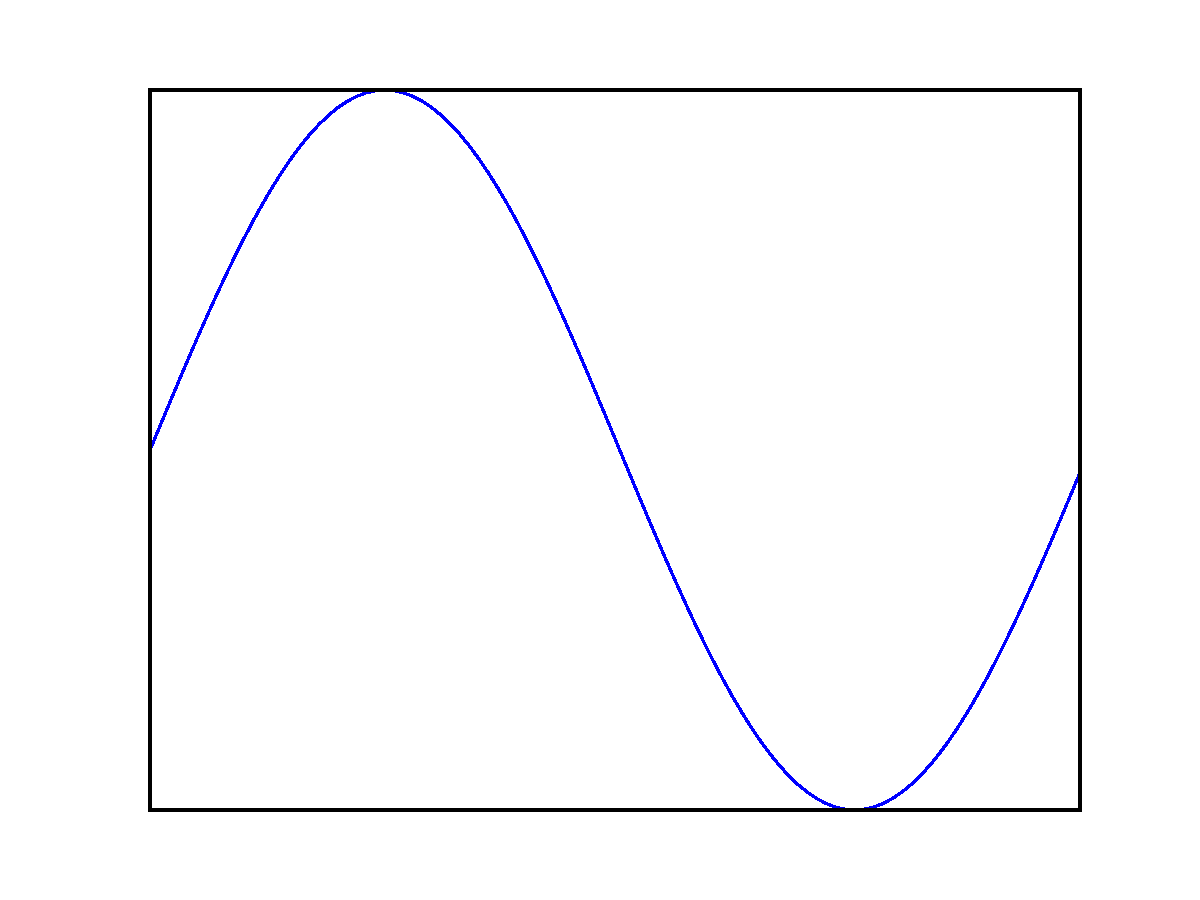
\includegraphics[scale=0.2]{figures/1d_manifold.pdf}
		}
		\end{subfloat}~
		\begin{subfloat}[$\mathbb{R}^2 \rightarrow \mathbb{R}^3$]{%
			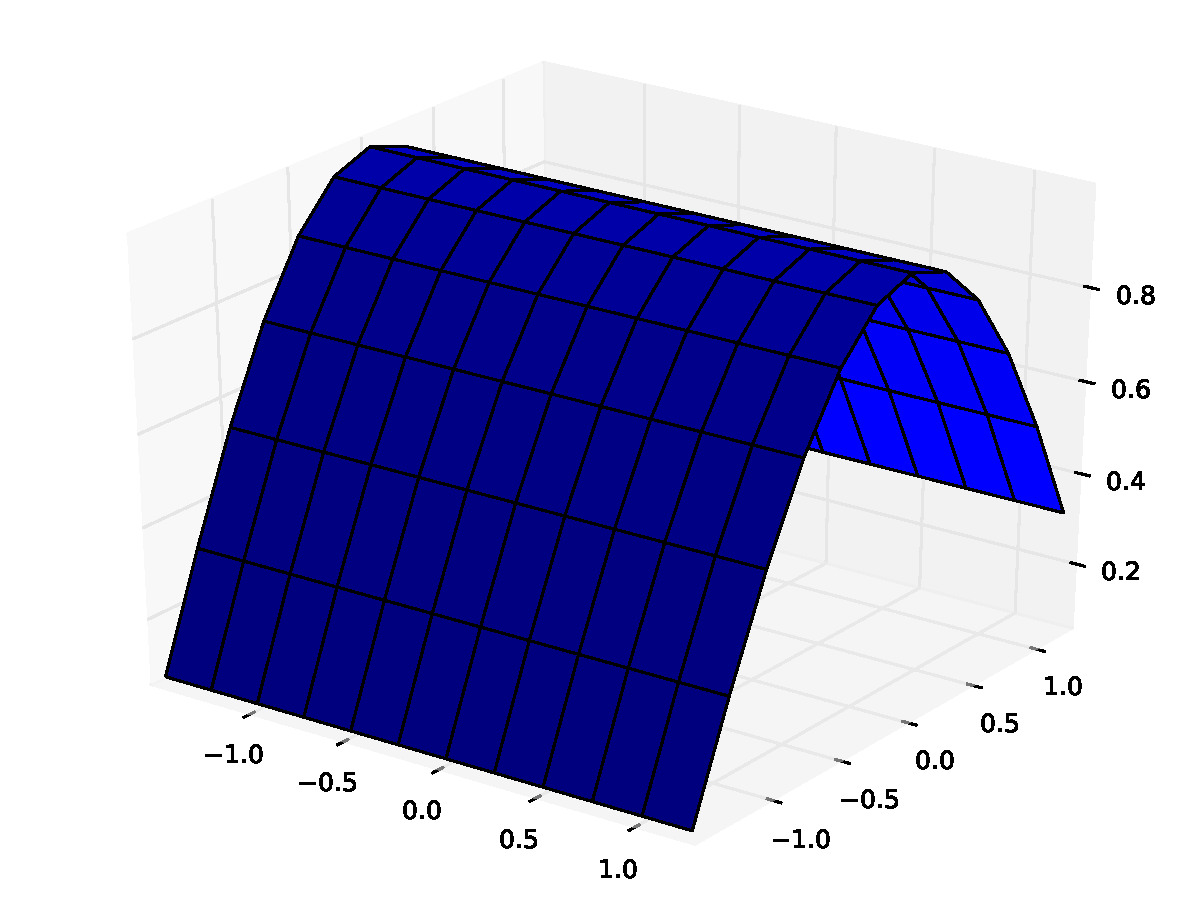
\includegraphics[scale=0.225]{figures/2d_manifold.pdf}
		}
		\end{subfloat}
	\end{center}

	\caption{Manifolds Embedded in Higher-Dimensional Space}
	\label{fig:manifolds}
\end{figure}

TODO: lead this back to BINNING W/ PYRAMID TREE


\section{Suitability of Dimension Reduction Techniques}

The Pseudo-Pyramid Tree and Pyramid Tree both produce a \textit{static} decomposition of the underlying data space through the use of dimension reduction. They do not \textit{adapt} to the distribution of the input data by modifying the amount or size of bins. With dynamic data, where one does not know the distribution of the data in advance, these approaches are severely limited. This is shown by the empirical results from this project; the performance of these two structures on the real datasets is vastly inferior to the point $kd$-tree, a simple and well-established technique.

Adaptive variants of the Pyramid Tree exist, such as the Extended Pyramid-Technique \cite{pyramid-tree} and IMinMax($\theta$) \cite{iminmax}. However, the \textit{cost} of adapting such structures limits their usefulness. For example, the Extended Pyramid-Technique moves the centre of the data space to be the median point. Doing so means that the entire structure must be rebuild, because each stored point may be hashed to a different value after the data space is moved. For large $n$ this has a massive impact on performance. Suppose the structure stores a million points and then has to adapt -- a million points must be re-inserted. IMinMax($\theta$) was implemented in this project, but the performance was still poor despite it adapting to the dataset, due of the rebuilding procedure. For this reason, it has not been covered in detail in this report and the project did not explore adaptive dimension reduction techniques any further.

The $kd$-tree can be considered an adaptive technique because the decomposition of the data space depends on the points being stored, and not just the underlying data space. Despite the structure performing worse on highly skewed data like the astrophysics dataset, it can still process the data reasonably quickly. Bear in mind this is without \textit{any} major optimisations on the implementation and with no exploration of the numerous $kd$-tree variants that have been developed.

The empirical performance timings has lead the author of this report to conclude that techniques which perform a static decomposition of the data space are \textit{not} suitable for dynamic data. The supplementary theoretical analysis has shown that data generated by mapping continuous domains mapped to higher-dimensional ranges are especially a challenge for structures that cannot adapt, due to the highly clustered and skewed distributions of points that result from such a mapping. Most dimension reduction techniques are also not recommended, because the cost of adapting them to changing data distributions is too high. Index structures which can adapt to different distributions of data \textit{as} points are inserted, that require much less cost, appear to offer. Examples of such structures include the KDB-tree and splay quadtree (see Sections \ref{sec:recursive-partition-structures} and \ref{sec:history-sensitive-structures}).

\section{New Hypothesis}

TODO: new hyp being made. JUSTIFY AND THEN DESCRIBE IT

\paragraph{\textbf{HYPOTHESIS:}} TODO

TODO: beyond scope of project to prove it